\chapter{Fluent仿真与硬件系统}
	本课题围绕“超声速射流流场参数测量”与“CO$_2$相变机制”两个核心研究问题，建立了以实验测量为主、仿真模拟与理论分析为辅的研究方法体系。本章首先介绍Fluent流场仿真结果，为后续实验提供工况依据和验证真值；然后详细介绍各硬件子系统的设计与搭建，包括射流发生系统、TDLAS光路系统、纹影系统、位移扫描系统和数据采集系统。
	\subsection{Fluent流场仿真}
	\subsubsection{计算模型与边界条件}
	CFD仿真采用二维轴对称模型，计算域尺寸为轴向100~mm、径向40~mm，喷嘴出口位于轴向坐标$z=0$处。网格为结构化四边形网格（ICEM CFD生成），壁面附近加密（$y^+<1$），总网格数约5万。边界条件设置如下：
	\begin{itemize}
		\item 进口：压力入口，总压0.5~MPa，总温300~K；
		\item 出口：压力出口，静压0.1~MPa；
		\item 壁面：无滑移、绝热边界；
		\item 工质：纯CO$_2$，理想气体可压缩模型；
		\item 湍流模型：SST $k$-$\omega$（对射流剪切层和激波捕捉性能良好）；
		\item 求解器：基于压力的耦合求解器（Coupled算法），伪瞬态加速收敛；
		\item 离散格式：二阶迎风格式（动量、能量、湍流方程）；
		\item 收敛判据：各方程残差$<10^{-4}$，且出口流量监测值稳定。
	\end{itemize}
	\subsubsection{仿真结果}
	图\ref{fig:fluent_temp}—\ref{fig:fluent_vel}分别给出了CFD计算得到的温度场、压力场和速度场云图。
	\begin{figure}[H]
		\centering
		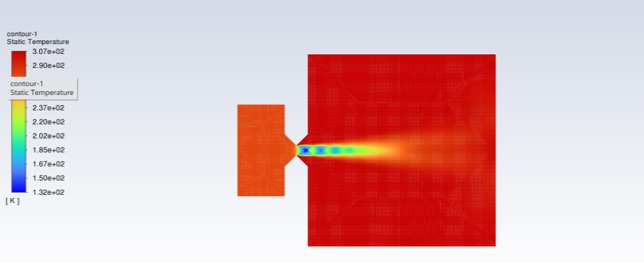
\includegraphics[width=0.8\textwidth]{figures/fig20.png}
		\caption{CFD计算的温度场结果}
		\label{fig:fluent_temp}
	\end{figure}
	\begin{figure}[H]
		\centering
		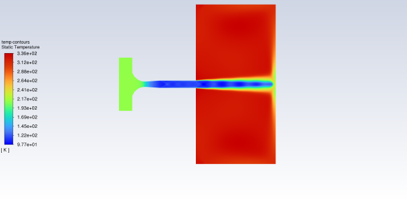
\includegraphics[width=0.8\textwidth]{figures/fig22.png}
		\caption{CFD计算的压力场结果}
		\label{fig:fluent_pressure}
	\end{figure}
	\begin{figure}[H]
		\centering
		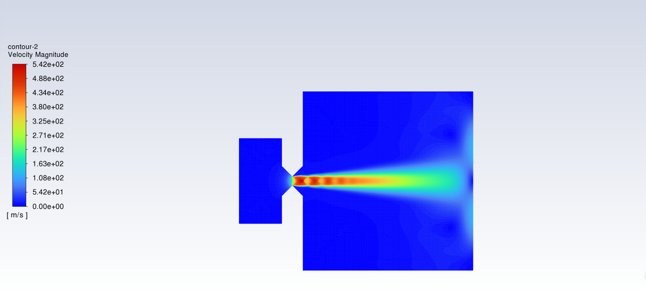
\includegraphics[width=0.8\textwidth]{figures/fig21.png}
		\caption{CFD计算的速度场结果}
		\label{fig:fluent_vel}
	\end{figure}
	仿真结果清晰显示了马赫盘、桶形激波和膨胀扇等典型欠膨胀射流结构特征。马赫盘位于$z\approx3.0$~mm处，射流核心区温度约260~K。提取沿轴线（$z=0\sim50$~mm）和马赫盘附近截面的温度、压力、密度径向分布，用于：
	\begin{enumerate}[label=(\arabic*)]
		\item 预估射流核心区温压范围，指导光谱仿真参数设置；
		\item 作为Abel反演算法的输入真值，验证反演精度；
		\item 与实验纹影图像对比，验证射流宏观结构。
	\end{enumerate}
	\subsection{射流发生系统}
	射流发生系统采用“小孔射流+大气膨胀”方案产生欠膨胀超声速射流。核心设备包括高压气源、混合腔体、小孔喷嘴及气路控制组件。
	\subsubsection{气源与工质}
	实验所用工质为纯CO$_2$（纯度99.9\%）和N$_2$（纯度99.9\%），分别由40~L高压气瓶供给（CO$_2$最高压力6~MPa，N$_2$最高压力9~MPa）。各气瓶出口配置两级减压阀（上游耐压15~MPa，减压范围0-1~MPa），经不锈钢管接入混合腔体。每条支路独立配备流量计与针阀用于精确控制工质混合比例与流量。
	\subsubsection{混合腔体}
	混合腔体为自主设计的铝制正方腔体（边长200~mm，容积约4~L），进气管路经腔体侧部引入，在腔体内实现CO$_2$与N$_2$的均匀混合。腔体内部安装压力传感器（量程0-1~MPa，精度±0.25\% F.S.）和K型热电偶（精度±0.5℃），实时监测腔体稳态压力与温度，确定射流前的状态参数。
	\subsubsection{小孔喷嘴}
	喷嘴采用304不锈钢材质，加工喉部直径分别为1~mm、2~mm、5.5~mm，出口锥角15$^\circ$。喷嘴与混合腔体通过螺纹连接，更换时保持同轴度。加工完成后使用ALICAT 1000SLM流量计进行了流量测试，发现小孔径喷嘴存在加工精度偏差：1~mm喷嘴在0.5-0.6~MPa压力下理论流量为29.9-33.5~L/min，实测流量为46-54~L/min，偏差超过50\%。分析认为主要原因是微小孔加工中喉部实际面积偏大及内壁粗糙度过高。针对该问题，使用800\#、1200\#、2000\#砂纸逐级打磨喷嘴内壁和出口端面，最后用氧化铝抛光液进行机械抛光，将1~mm喷嘴的实测流量提升约8\%，更接近理论值，纹影观察射流边界明显更清晰。
	\subsection{TDLAS光路系统}
	\subsubsection{激光器与控制器}
	激光源为2.7~$\mu$m分布式反馈量子级联激光器（QCL，中心波长2705~nm，典型输出功率7~mW），由模块化激光二极管控制器（SRS LDC3916374，16通道，GPIB接口）驱动。控制器参数设置范围：LD电流上限180~mA，电压上限2.5~V，TEC温度范围0-50$^\circ$C，TEC最大电流1.4~A。激光器与控制器通过DB9电缆连接，确认互锁回路闭合后方可开启输出。控制器通过GPIB-USB适配器与上位机通信，编程环境为Python 3.9 + PyVISA。
	\subsubsection{探测器}
	探测器为碲镉汞（HgCdTe）光伏探测器（Vigo System PVI-2TE-8），响应波长范围2-12~$\mu$m，探测率$D^* = 2.5\times10^9$ cm$\cdot$Hz$^{1/2}$/W，响应时间小于100~ns，前置放大器带宽5.5~MHz。探测器输出信号经50$\Omega$阻抗匹配后接入示波器或数据采集卡。探测器需在-20$^\circ$C环境下工作（内置四级热电制冷器），由专用温度控制器驱动。
	\subsubsection{光路布局}
	TDLAS光路采用双光路耦合设计（图\ref{fig:optical_setup}）：532~nm可见光（绿光激光笔，50~mW）用于光路指引与姿态校准，2.7~$\mu$m中红外激光用于核心测量。两束光通过硒化锌窗口片（直径20~mm，厚度3~mm，透射率$>$95\%@2.7$\mu$m）实现同轴耦合，依次穿过两个同轴小孔光阑（孔径1~mm，间距500~mm）滤除杂散光并校准同轴度。
	\begin{figure}[H]
		\centering
		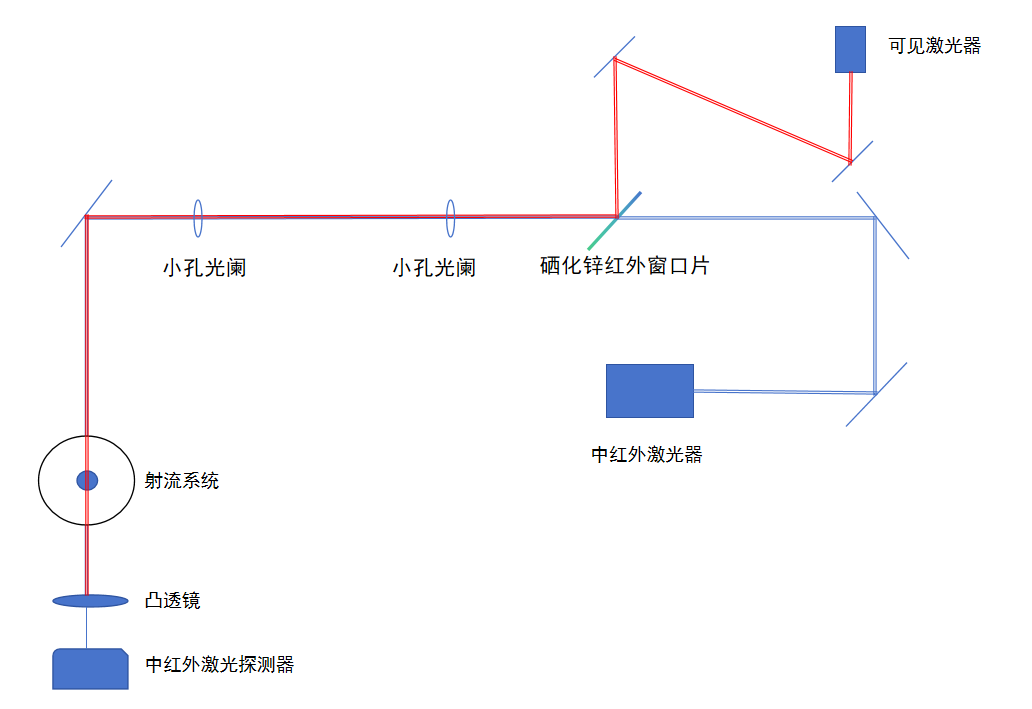
\includegraphics[width=0.9\textwidth]{figures/fig5.png}
		\caption{TDLAS光路布局示意图}
		\label{fig:optical_setup}
	\end{figure}
	光路元件包括：
	\begin{itemize}
		\item 平面金镜（Thorlabs PF10-03-P01，直径25.4~mm，镀保护金膜，反射率$>$96\%@2.7$\mu$m），共6面；
		\item 氟化钙平凹透镜（$f=-40$~mm）与平凸透镜（$f=100$~mm、$f=150$~mm）组合，用于光斑聚焦；
		\item 硒化锌红外窗口片（直径20~mm，厚度3~mm），安装于混合腔体出口，透射率$>$95\%@2.7$\mu$m。
	\end{itemize}
	\subsubsection{激光器工作参数}
	经系统调试，锁定激光器最优工作参数：TEC温度44.5$^\circ$C（温度稳定性$\pm$0.01$^\circ$C），偏置电流110~mA，调制信号频率1000~Hz正弦波，调制幅度0.85~Vpp。调制幅度与电流的换算关系为$I_{\rm pp} = (I_{\rm FS}/10\mathrm{V}) \times V_{\rm pp}$，其中$I_{\rm FS}=1.5$~A，$V_{\rm pp}=0.85$~V，对应的峰值电流变化为127.5~mA，叠加偏置后总电流峰值约173.75~mA，低于激光器上限180~mA。
	\subsection{纹影系统}
	纹影系统用于射流宏观结构可视化。系统采用反射式Z型布局（图\ref{fig:schlieren_setup}），核心参数：
	\begin{itemize}
		\item 光源：LED灯珠（波长530~nm，功率5~W），经聚光镜和狭缝（宽度0.5~mm）形成点光源；
		\item 凹面镜：口径150~mm，焦距1500~mm（镀保护银膜，反射率$>$95\%），共两面；
		\item 刀口：可调宽度，置于第二凹面镜焦点处，用于切割偏折光线；
		\item 相机：黑白工业相机（分辨率1920$\times$1200，帧率60~fps），配50~mm定焦镜头。
	\end{itemize}
	纹影系统空间分辨率约50~$\mu$m，时间分辨率由相机帧率决定（最短曝光时间1~ms），足以捕捉马赫盘和激波胞等瞬态结构。实验时刀口切割量调节至图像对比度最佳，背景扣除采用无射流状态下的平均图像。
	\begin{figure}[H]
		\centering
		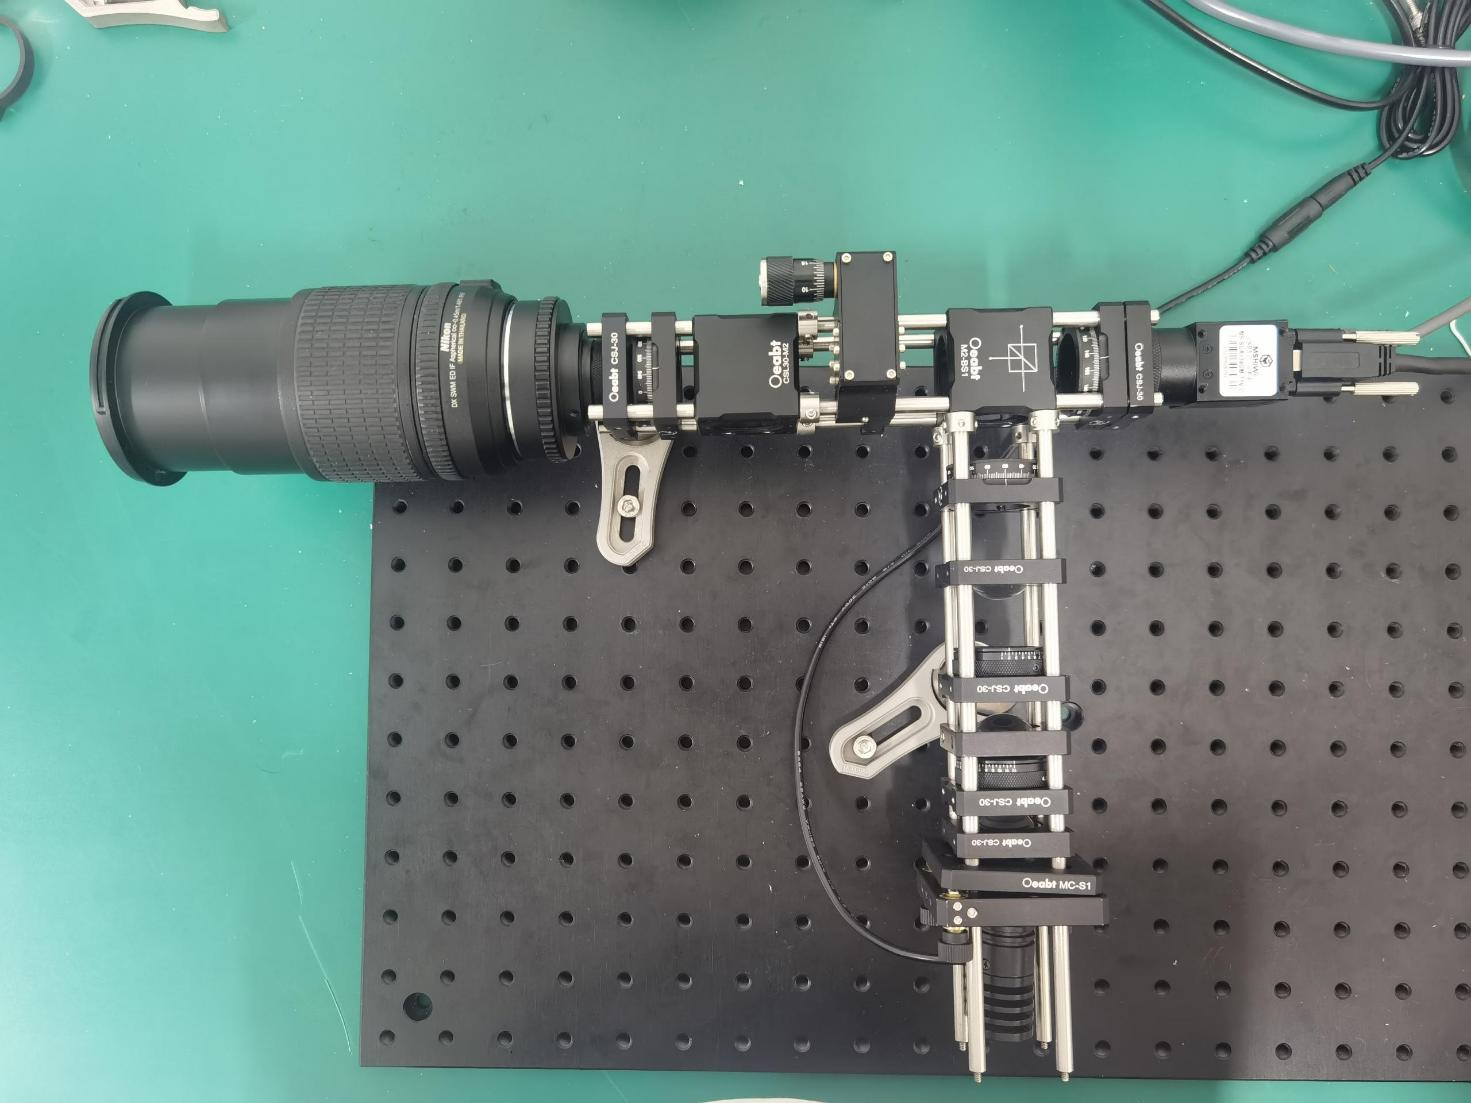
\includegraphics[width=0.8\textwidth]{figures/fig6.png}
		\caption{反射式纹影系统光路布局}
		\label{fig:schlieren_setup}
	\end{figure}
	\subsection{位移扫描系统}
	位移扫描系统由伺服电机、精密导轨和控制器组成，用于实现喷嘴在二维平面内的自动定位。
	\begin{itemize}
		\item 伺服电机：超川伺服电机（额定扭矩1.27~Nm，编码器分辨率17位），位置控制模式；
		\item 精密导轨：THK线性导轨（行程100~mm，重复定位精度$\pm$0.01~mm）；
		\item 控制器：超川CD系列伺服驱动器，通过RS485总线与上位机通信；
		\item 控制软件：Python 3.9 + pySerial库，控制帧格式为“目标位置+速度+加速度”，通信波特率115200~bps。
	\end{itemize}
	扫描策略为“步进-采集”模式：喷嘴移动至目标位置后停顿1~s（机械振动衰减），然后开始光谱采集；采集完成后移动至下一位置。单点定位时间约3~s（含加减速）。使用高精度水平仪完成试验台调平（X方向偏差0.05~mm/m，Y方向偏差0.08~mm/m），调平后扫描定位重复性预计提升约30\%。电机运行时的电磁干扰问题已确认，当前采取“移动到目标位置后停转并关闭使能，再进行采集”的策略。
	\subsection{数据采集系统}
	数据采集系统基于Red Pitaya STEMlab 125-14开发板（图\ref{fig:redpitaya_setup}），核心参数：
	\begin{itemize}
		\item ADC：14位分辨率，125~MSa/s采样率，双通道同步采集；
		\item FPGA：Xilinx Zynq 7010（ARM Cortex-A9双核 + Artix-7 FPGA）；
		\item 模拟输入：$\pm$1~V / $\pm$20~V两档可切换，输入阻抗1~M$\Omega$；
		\item 通信接口：千兆以太网，SCPI协议远程控制；
		\item 同步方式：自触发同步采集。
	\end{itemize}
	软件层面采用Python 3.9 + PyVISA库通过SCPI协议控制开发板。数据采集参数：每个采样点采集1000个周期，每周期15000点，软件累加平均500次，单点采集时间约2~s（含传输和平均运算）。DMA方式使单点采集时间优化至约0.3~s。
	\begin{figure}[H]
		\centering
		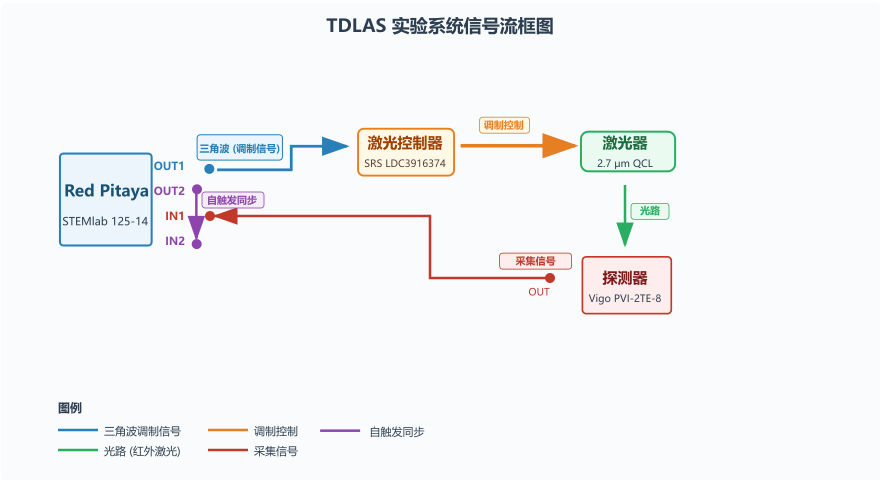
\includegraphics[width=0.6\textwidth]{figures/fig7.png}
		\caption{Red Pitaya数据采集系统框图}
		\label{fig:redpitaya_setup}
	\end{figure}
	\textbf{自触发同步方案}：为解决触发抖动导致多周期波形无法对齐的问题，采用“开发板DDS产生调制信号 + 同一主时钟触发采集”的自触发方案。该方案的关键优势在于：激光调制与ADC采集共用一个125~MHz主时钟，不存在时钟异步问题，相邻周期波形的吸收峰位置偏差$<0.1$采样点，远优于外部触发方式（偏差约3-5个采样点）。平均后随机噪声显著降低，吸收峰位置清晰可辨，SNR从约5提升至约30，验证了平均方案的有效性。
	% ==================== 第四章 光谱仿真与纹影诊断 ====================

